\utsection{OpenBSC}{Stefan Giggenbach}\label{sec:openbsc}

\subsection{Überblick}

Bei OpenBSC handelt es sich wie bei OpenBTS um Open Source Software. Der große Vorteil von OpenBSC liegt in der \textit{network in the box} (nitb) genannten Version, die ohne zusätzliche Software-Komponenten den Betrieb eines GSM-Netzwerks ermöglicht. Dadurch war es möglich zu einem sehr frühen Zeitpunkt im Projekt ein GSM-Netzwerk mit Handover-Funktionalität zu betreiben und die Abläufe zu analysieren (siehe Kapitel \ref{sec:analyse}). Abbildung \ref{fig:openbscarch} zeigt die umgesetzte Architektur.

\begin{figure}[h!]
  \centering
  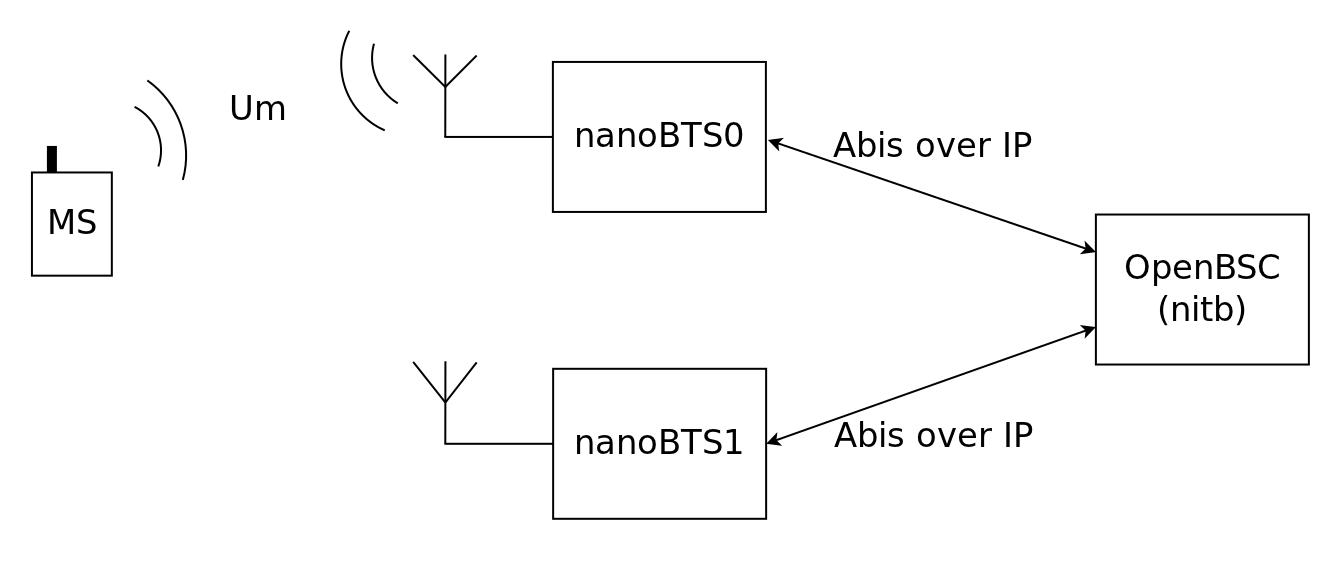
\includegraphics[width=0.9\textwidth]{img/openbscarch}
  \caption{OpenBSC Architektur}
  \label{fig:openbscarch}
\end{figure}

OpenBSC übernimmt nicht nur die Funktion des BSC sondern auch die des MSC. Die Teilnehmer Datenbanken HLR und VLR werden mit einer SQLite3 Datenbank realisiert. Wie in Abbildung \ref{fig:openbscarch} dargestellt werden zwei nanoBTS der Firma ip.access verwendet. Diese werden über zwei Abis-over-IP-Schnittstellen an OpenBSC angebunden. Mit dieser Architektur ist somit die Durchführung eines in Abschnitt \ref{sec:handover} beschriebenen Intra BSC Handover mit verhältnismäßig geringem Installations- und Konfigurationsaufwand möglich.

\subsection{Installation und Konfiguration}

Die Installation von OpenBSC ist ausführlich im Wiki des Projekts \cite{bib:buildopenbsc} dokumentiert. In diesem Abschnitt werden deshalb nur die wichtigsten Punkte der Installation und die Konfiguration des Systems für den Multi-BTS-Betrieb behandelt.

OpenBSC (nitb) besteht aus insgesamt drei Komponenten:

\begin{itemize}
 \item libosmocore - Die Kernbibliothek, die auch für andere Projekte (z.\,B. OsmoBTS) verwendet wird.
 \item libosmo-abis - Die Bibliothek zur Umsetzung der Abis- und Abis-over-IP-Schnittstelle.
 \item openbsc - Die eigentlich OpenBSC-Software, die auch die nitb Version enthält.
\end{itemize}

Nach der Kompilierung und Installation dieser drei Komponenten können die beiden nanoBTS, die sich im selben IP-Netzwerk befinden müssen, konfiguriert werden. Dazu werden die zwei Anwendungen \lstinline{./ipaccess-find} und \lstinline{./ipaccess-config} im Verzeichnis \lstinline{openbsc/src/ipaccess} benötigt. Die Verwendung der beiden Befehle und die benötigten Parameter zur Konfiguration werden ebenfalls im Wiki des Projekts \cite{bib:ipaccess} erläutert. Die bei der Konfiguration der nanoBTS vergebene UnitID (diese kann frei gewählt werden) ist ein wichtiger Parameter, der für die im Folgenden beschriebene Konfiguration von OpenBSC benötigt wird.

Um den Betrieb beider nanoBTS und die Handover-Funktionalität von OpenBSC zu aktivieren, muss die Konfigurationsdatei von OpenBSC modifiziert werden. Als Grundlage wird die Beispielkonfiguration \lstinline{openbsc/doc/examples/osmo-nitb/nanobts/openbsc.cfg} verwendet. Listing \ref{lst:config} zeigt auszugsweise die wichtigsten Inhalte der modifizierte Konfigurationsdatei.

\begin{lstlisting}[label=lst:config,caption=OpenBSC Konfigurationsdatei (Auszug)]
!
! OpenBSC (0.10.1.40-2935) configuration saved from vty
.
network
 network country code 262
 mobile network code 98
 .
 handover 1
 .
 bts 0
  type nanobts
  band DCS1800
  cell_identity 0
  .
  ip.access unit_id 42 0
  .
  trx 0
   rf_locked 0
   arfcn 846
   nominal power 23
   max_power_red 22
   .
 bts 1
  type nanobts
  band DCS1800
  cell_identity 1
  .
  ip.access unit_id 43 0
  .
  trx 0
   rf_locked 0
   arfcn 840
   nominal power 23
   max_power_red 22
   .
\end{lstlisting}

%TODO: Kurze Beschreibung der Modifikationen

Anschließend kann das komplette System mit dem Befehl \lstinline{./openbsc/src/osmo-nitb/osmo-nitb} gestartet werden. Ein Handover kann bei aktiver Verbindung durch Veränderung der Position oder durch ausreichende Abschirmung der Mobile Station ausgelöst werden. Die Analyse der Handover wird in Kapitel \ref{sec:analyse} detailliert beschrieben.
